\documentclass[../pfc.tex]{subfiles}

\begin{document}

	
	\section{Construcción}
	
	Para la implementación en un principio las metodologías ágiles no marcaban ninguna pauta más allá de que todo lo que no está terminado al 100\% no está terminado y por otro lado que siempre hay que entregar al cliente un trabajo con la máxima calidad posible, aunque quizá la más importante fue que la propiedad del código es colectiva, ya no hay más código mio o código tuyo y tenemos responsabilidades y atribuciones sobre nuestras parcelas, el código es del equipo entero y todo miembro puede y debe mejorar el mismo si observa y detecta un error. Seguimos la regla del boy scoutt de Clean Code\cite{cleancode}, que nos dice "Deja el campamento más limpio de como lo encontraste".\\*
	
	Después de un tiempo de maduración de las mismas surgieron técnicas y disciplinas, algunas en el seno de alguna de estas metodologías (XP sobre todo) y algunas se incorporaron rápidamente desde el movimiento Craftmanship software \cite{manifestocraft} que tiene una filosofía similar aunque más cercana y centrada en el proceso de construcción en sí que en el resto del proceso de desarrollo del proyecto o producto. Estas técnicas son Pair Programming, TDD, Code Reviews y algunas centradas en la mejora del equipo en todos los proyectos como puedan ser Code Retreats, Katas, Koans, etc. todas estas técnicas y disciplinas hoy en día se consideran tan apegadas a las metodologías ágiles que prácticamente se confunden con las mismas cuando hablamos del proceso de implementación.\\*
	
	Lo que si existe es la idea del visual management, o tener algún tipo de respaldo visual del estado de un proyecto. Para esto existen pizarras en las que mediante el uso de tarjetas, imanes, post its, imágenes e incluso avatares de los miembros del equipo, permiten que cualquier persona interesada en el proyecto con solamente dar un vistazo a la pizarra vea el estado del sprint actual, en que trabaja cada miembro del equipo, el estado del backlog, las historias completadas, y demás información que cada equipo adapta a sus necesidades.\\*
	
	Recordemos que la idea es que el equipo y el product owner se sientan cómodos con la metodología y la adapten a sus necesidades o idiosincrasia, teniendo en cuenta que no hay balas de plata que sirvan para todo y arreglen los problemas de la noche a la mañana.\\* 
	
	Existen también multitud de utilidades de software que permiten esto mismo para equipos remotos o para aquellos que no les es posible disponer de una pizarra física. Esta ha sido la opción utilizada por nosotros a través de la aplicación web Trello, debido a la composición distribuida tanto del equipo, como de cada uno de los diferentes product owner de parte de la AECC\\*
	
	\begin{figure}[H]
		\centering
		
\includegraphics[width=0.5\linewidth]{../images/TrelloLogo}
		\caption{Logo de la aplicación Trello}
		\label{fig:trello}
	\end{figure}
	
	Esta app permite el uso de la pantalla como si de una pizarra electrónica se tratase, no es necesario compartir un espacio físico para ello y de manera sencilla se puede compartir con todos los miembros que forman parte del equipo. Para nuestro propósito la dividimos en diferentes columnas que representarán los estados de una historia de usuario y además algunas zonas para colocar una imagen del burndown, el estado de animo del equipo y del product owner. La explicación de las columnas y como adaptamos nuestra manera de desarrollar y de llevar scrum a Trello se hace más abajo.\\*
	
	\begin{figure}[H]
		\centering
		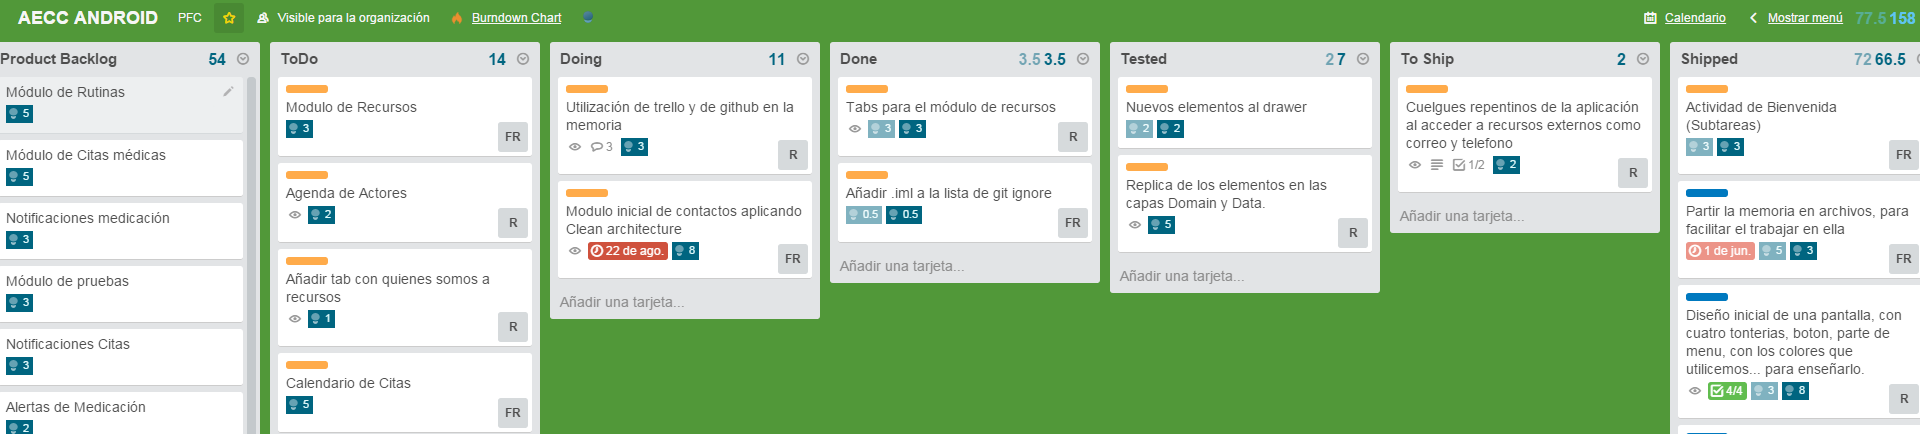
\includegraphics[width=1\linewidth]{../images/trellocomphorizontal}
		\caption{Vista general de la columnas de scrum en Trello}
		\label{fig:trelloComp}
	\end{figure}
	
	Las columnas que definimos como estados para las historias de usuario fueron:\\*
	
	\begin{figure}[H]
		\centering
		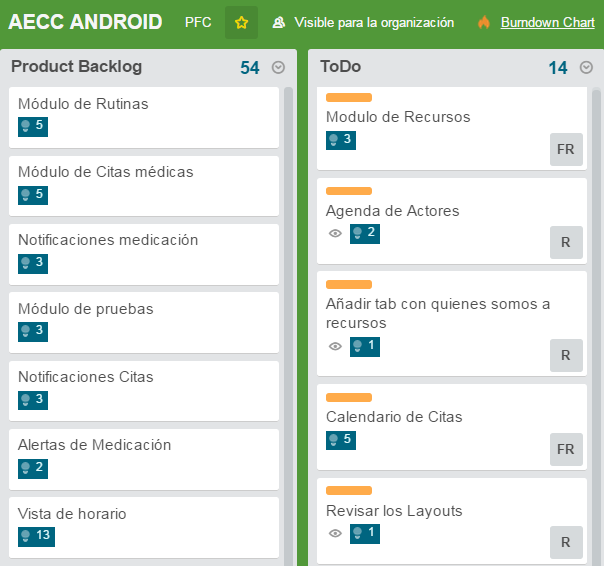
\includegraphics[width=0.6\linewidth]{../images/pbacklog_todo}
		\caption{Detalle de las columnas product backlog y ToDo}
		\label{fig:trelloBackDo}
	\end{figure}
	
	\begin{itemize} 
		\item Product Backlog, es el backlog de la aplicación del que se habló en el Capitulo 3. Debe estar priorizado para que el equipo tenga una visión aproximada de los intereses del product owner en futuros sprints, pero el equipo ha de ser consciente de que esto puede ser modificado por el product owner en cualquier momento. La priorización de las historias y dada la facilidad con la que Trello nos permite mover las tareas en la misma columna y entre columnas se realizo de la siguiente manera, la más prioritaria es la que ocupa el primer lugar en esa columna, y es con la que se empezará una vez se le asigne un sprint.
		\item Sprint Backlog o ToDo, son las tareas del sprint en curso o por hacer. Pueden estar priorizadas por el product owner (del modo que hemos comentado antes) para que el equipo tenga cierta idea de lo que es más valioso para el, pero el equipo es libre del orden de implementación de las historias en un sprint, en esta columna en un principio se encuentran todas las tareas que forman parte de ese sprint, y será el principal punto de entrada a la hora de asignar tareas al equipo. 
		
		\begin{figure}[H]
			\centering
			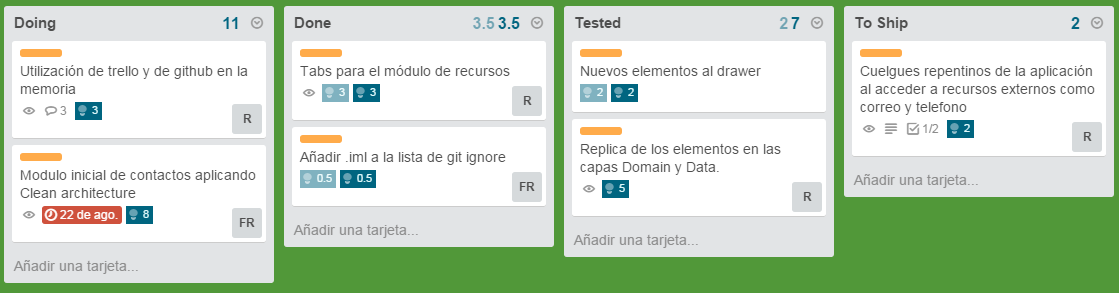
\includegraphics[width=1\linewidth]{../images/do_done}
			\caption{Detalle de las columnas Doing, Done, Tested y To Ship}
			\label{fig:trelloDDTT}
		\end{figure}
		
		\item Doing, es la columna de las historias que actualmente se encuentran en proceso de implementación por algún miembro del equipo.
		\item Done o ToTest, tareas que el equipo ha dado por terminadas con sus test unitarios y prueba de aceptación o definition of done completado, pero no por alguien ajeno al desarrollo de la misma, suele ser el mismo miembro del equipo asignado a la tarea el que la pasa a esta columna. 
		\item Tested, alguien ajeno al desarrollo de la historia de usuario ha testado el criterio de aceptación de la historia, esto puede ser llevado a cabo por el scrum master o algún miembro del equipo designado para ello, al estar nuestro equipo formado por dos personas solemos cruzar la comprobación de las mismas. 
		\item ToShip, historias que se han probado por alguien ajeno a quien la desarrolló, pero que aun no han sido entregadas o desplegadas para demo o validación por el product owner, hay funcionalidades que se acaban pero que por alguna razón no se quieren llevar a la demo en curso y permanecen en esa columna durante algún tiempo.
		
		\begin{figure}[H]
			\centering
			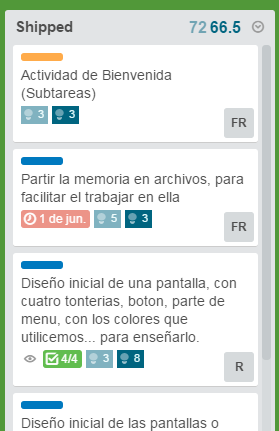
\includegraphics[width=0.5\linewidth]{../images/shipped}
			\caption{Detalle de la columna Shipped}
			\label{fig:trelloSipped}
		\end{figure}
		
		\item Shipped, historias que fueron entregadas o desplegadas en otros sprints o en una demo, idealmente no deberían salir de esta columna ya que como se dice han sido validadas por el product owner, pero pudiera ser que se presenten errores en test de regresión al añadir nueva funcionalidad. En ese caso pasarían al Product Backlog para el siguiente sprint como historia de defecto, tal y como esté acordado por el equipo.
		
	\end{itemize}
	
	La transición de las historias que se escriben en tarjetas físicas a las historias virtuales con las que trabajamos en Trello se ha realizado de una forma sencilla.
	La tarjeta consta de varias partes como son el título, los puntos de Historia que le asignamos tras previa votación (debajo se encuentran los que ha llevado acabarla una vez este hecha), el miembro del equipo o los miembros que se van a encargar de su elaboración, la descripción, Subtareas que se pueden añadir en forma de checks, comentarios,...\\*
	
	Los puntos de historia estimados y los completados, nos ayudan a la hora de estimar el ¿Cómo vamos? ya que nos va haciendo un recuento sobre la columna de los que quedan y los que se han hecho. También se le puede añadir a la tarea una fecha de vencimiento a modo de "Dead Line", para fijar una fecha de antemano en la que esa tarea debería estar completada y en la columna "ToShip".\\*
	 
	Otra de las funcionalidades que nos aporta Trello, es la suscripción, algo muy útil a la hora de recibir un email con su resolución, o cambio de columna y que facilita el flujo de trabajo sobremanera.\\*
	El etiquetado lo utilizamos sobre todo para indicar a que sprint pertenece la tarea y a la hora de realizar búsquedas por la misma etiqueta las agrupa, permitiendo revisar las que pertenecen al mismo.
	
		\begin{figure}[H]
			\centering
			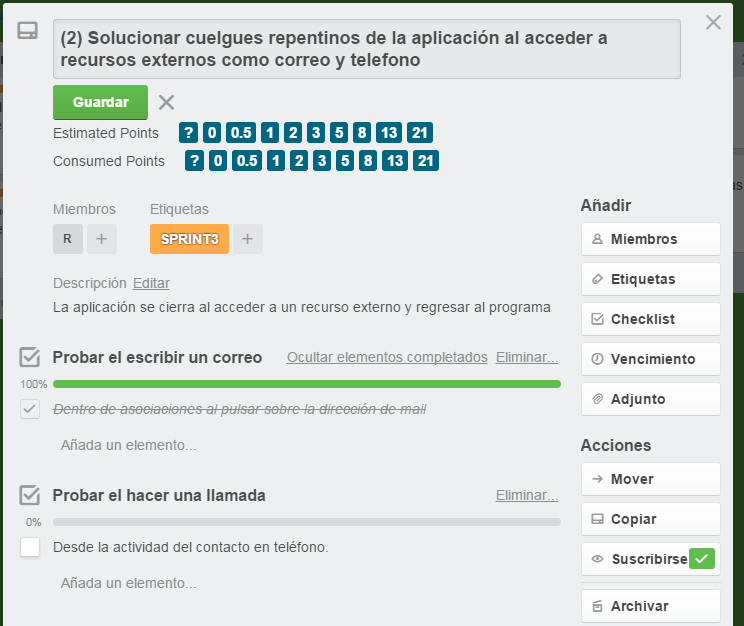
\includegraphics[width=1\linewidth]{../images/tarea2}
			\caption{Implementación de las Historias de usuario en Trello}
			\label{fig:tareaTrello}
		\end{figure}
		
	Las etiquetas bajo las que señalamos el sprint en el que se encuentra la tarea, nos ayudan a la hora de realizar las búsquedas y son útiles para repasar los puntos de historia que se han completado en ese sprint y poder planificar de manera más eficiente los siguientes. Ya que con la finalización de cada sprint, hay una DEMO y esta debería incluir todas las funcionalidades que en principio se plantearon incluir.
		
		\begin{figure}[H]
			\centering
			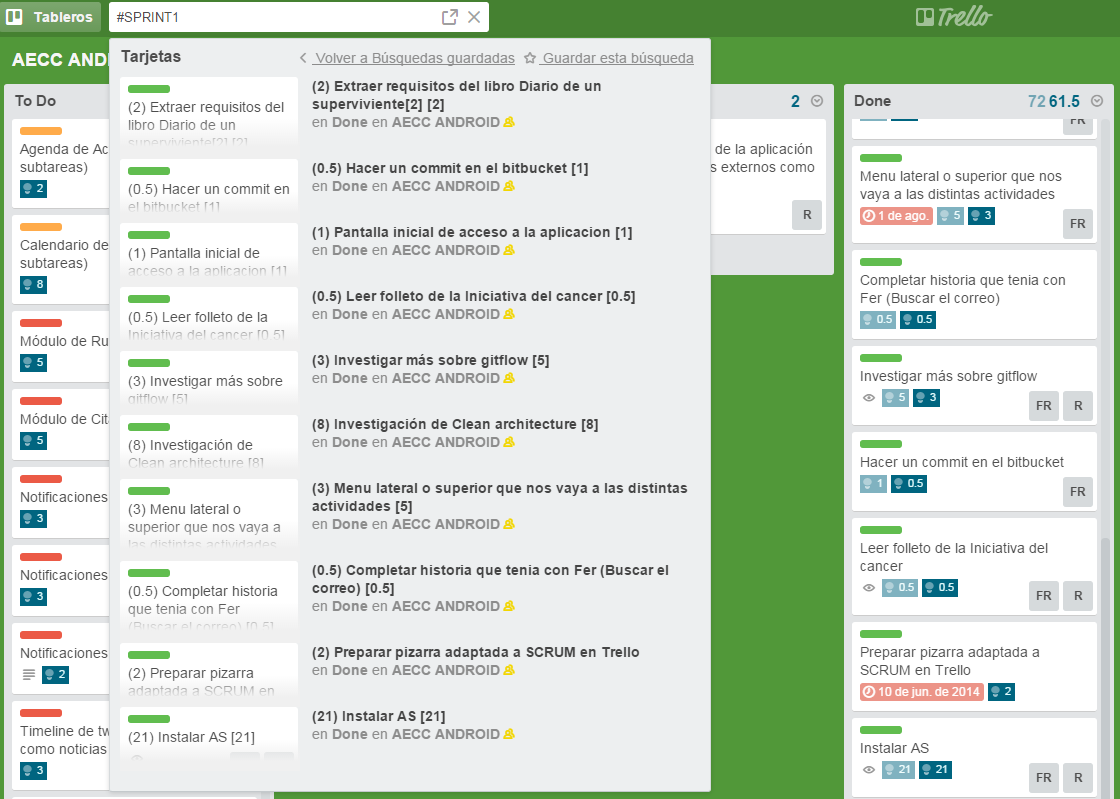
\includegraphics[width=1\linewidth]{../images/sprints2}
			\caption{Agrupación de tareas por sprints}
			\label{fig:sprints}
		\end{figure}

	En todo momento las historias avanzan hacia la derecha de la pantalla, nunca hacia la izquierda. Cada miembro del equipo solo podía estar dedicado a una tarea, ocasionalmente dos miembros del equipo pueden colaborar en la realización de una d
	tarea compleja, o usando la técnica de pair programming. 
	
	
	\section{Plan de desarrollo}
	Pasos para el desarrollo de la aplicación móvil "Diario de un Superviviente":\\
	
	\textbf{Idea Inicial}
	
	Partimos de la 'idea' conformada junto a la AECC de una aplicación Android  que permitiese a los enfermos de cáncer llevar de una manera mucho mas sencilla el control de las acciones que acontecen de manera rutinaria en su día a día, tales como la toma de medicamentos, asistencia a citas médicas, control de síntomas y pruebas, rutinas diarias beneficiosas.
	
	Para ello la AECC puso a nuestra disposición un folleto que forma parte de esta iniciativa, pero que dadas sus características físicas se que da algo corto en su planteamiento.\\
	
	\textbf{Captura de requisitos}
	
	El proyecto debe estar bien definido, tanto sus objetivos como las funcionalidades que se requieren para que cumpla su cometido. Cuanta mejor definido esté más cerca estaremos de cumplir sus objetivos.
	
	Está tarea, se ha realizado estudiando de manera pormenorizada la documentación que puso a nuestra disposición la AECC dividiendo en partes bien diferenciadas las funcionalidades de cada una de las partes de las que se compone esta documentación.
	
	A través del cruce de correos y de alguna que otra reunión presencial se han limado distintas formas de ver algunas partes.\\
	
		
	Con la definición del proyecto terminada, es necesario saber el tiempo que nos va a llevar en horas, por lo que hay que valorar el desarrollo. Para ello, será necesario contabilizar y estimar los plazos en horas que nos va a costar cada parte del proyecto. Tanto el plazo como el precio dependerán totalmente de las funcionalidades y del tipo de desarrollo elegido, pues no es lo mismo (ni se obtiene un proyecto de igual calidad) desarrollar apps nativas que híbridas, ni que el proyecto requiera de un complejo Backend orientado a móviles o no requiera siquiera esta parte.\\
	
	\textbf{Planificación} 
		
	Es la primera fase del desarrollo del proyecto. Consiste en tener un programa de trabajo con un desglose de todas las actividades que se van a realizar (desde el diseño hasta las pruebas finales), el plazo estimado de horas que se le va a dedicar cada una de ellas y estableciendo los medios humanos que se van a dedicar para alcanzar los objetivos que se hayan propuesto. En este proceso, que ha de ser continuo se han de reflejar\\
	
	-Equipos, programas, licencias etc que se vayan a emplear.
	
	-Requerimientos gráficos y fechas límite.
	
	-Necesidades que dependan del cliente (AECC) y fechas para tenerlos disponibles.
	
	-Cambios que puedan ocurrir durante el desarrollo de la app.
	
	Una buena planificación y su actualización es clave para el correcto desarrollo de la aplicación móvil y para su puesta en funcionamiento en la fecha prevista.\\  
	
	\textbf{Diseño UI/UX}
	
	Previo a la implementación es necesario tener totalmente definido el diseño estructural de la app y su comportamiento. Para ello hemos utilizado Photoshop para el diseño inicial, el cual nos mostrará el aspecto y la usabilidad de la aplicación.
	
	El diseño consiste tanto  en la confección del aspecto y usabilidad como en la correcta aplicación de las guidelines de diseño de Google de material design\cite(materialStructure),  además de la correcta adaptación a todas las densidades de pantallas (recordemos que por ejemplo Android tiene MDPI(160 DPI), HDPI(240 DPI), XHDPI(320 DPI), XXHDPI(480 DPI), XXHDPI (640 DPI) y su tratamiento para que sean aptas para la programación.\\
	

	\textbf{Desarrollo}
	
	Es la programación del proyecto. Esta fase se hará de acuerdo a la tecnología que se haya decidido emplear para cada plataforma de programación y los entornos de desarrollo empleados serán acordes con ello (Android Studio); recordemos que se pueden desarrollar apps nativas o híbridas , y llevará mayor esfuerzo de trabajo en función de lo anterior. A la vista de lo anterior el equipo de desarrollo, de una aplicación, por muy sencilla que sea, puede llegar a estar compuesto por 5 ingenieros informáticos (Android, iOS, Windows Phone, Backend, Frontend) y un diseñador, además del director del proyecto que coordine a todos ellos. De ahí que el coste de una app sea totalmente dependiente de la tecnología que empleemos en el desarrollo y de la complejidad del proyecto en sí.\\
	
	\textbf{Testing}
	
	Una vez desarrollada la app es necesario hacer un testing profundo de todas las partes del mismo. El testeo se puede dividir en:
	-Testeo funcional: para asegurar que la aplicación trabaja como debería y sigue todos los flujos debidos.
	-Testeo de rendimiento: para comprobar que el comportamiento de la aplicación bajo ciertas condiciones (múltiples peticiones de acceso simultáneas, poca cobertura, poca batería...) es el correcto.
	-Comprobaciones de fugas de memoria, cruciales en móviles pues los recursos son mucho más limitados que en programas para ordenadores de sobremesa. Para esta tarea se utilizan habitualmente programas automatizadores de tareas y programas que reportan el código de error, además del testeo manual intensivo.\\*
	
	\textbf{Distribución pre-lanzamiento}
	
	Previo a la subida a los markets de aplicaciones móviles se pueden hacer distribuciones de las aplicaciones móviles. En Android se puede hacer utilizando el entorno beta de desarrollo  Android disponible en la consola de desarrollador.\\*
	
	\textbf{Implantación y distribución}
	
	A la finalización del desarrollo, el último paso será subirlo a los markets correspondientes. Para este último paso habrá que firmar digitalmente las apps con la cuenta de desarrollador, compilar el paquete y subirlo a Google Play, así como preparar el resto de requisitos necesarios tales como las imágenes, logos, descripciones etc. Requeridos por los markets de apps.\\*
	A partir de este momento comienza la etapa de mantenimiento de la aplicación, y su escalabilidad, dependiendo de los requerimientos y necesidades futuras de los usuarios o del propio cliente en  nuestro caso de la AECC.
	
	Esperamos que aclare las dudas que podáis tener cuando penséis en desarrollar una aplicación móvil.
	
	\section{Versionado y Sincronización}

	El control de cambios y la gestión de la configuración son piezas claves en  el desarrollo de hoy en día, y los equipos deben poder confiar en un sistema que salvaguarde los cambios del código y que les permita compartir dichos cambios realizados en el ordenador local de cada integrante del equipo.\\*
	
	Es por esto que los sistemas de control de versiones y de gestión de la configuración han sido uno de los puntos claves en las infraestructuras de las empresas dedicadas a la producción de código. \\*
	
	En nuestro caso este pieza toma más importancia si cabe debido a que configuramos un equipo distribuido que se encuentra alejado en el espacio y que no siempre puede coincidir temporalmente para trabajar en el proyecto.\\* 
	
	De entre todos los sistemas de control de versiones existentes hoy día, por su capacidad y concepción distribuida desde su inicio nos decidimos por el sistema de control de versiones Git, usado en el desarrollo del kernel de Linux.\\*
	
	Así mismo necesitamos una red de salvamento por si alguno de los integrantes del equipo tenía que volver atrás en la versión de la aplicación que estaba manejando, crear una nueva version de la aplicación e incluso desestimar todos sus cambios y volver a una version más estable anterior y empezar desde ahí.\\*
		
	La necesidad de que fuese algo gratuito, que nos ofreciese suficientes garantías, tuviera una gran comunidad detrás y que pudiera integrarse de manera sencilla y compatible con Android Studio, ademas de que un funcionamiento y rendimiento alto serían deseables así como un acceso web serían características muy deseables en el sistema a utilizar.  
	
	\begin{figure}[H]
		\centering
		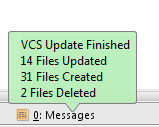
\includegraphics[width=0.4\linewidth]{../images/VCS}
		\caption{Integración de Git en Android Studio}
		\label{fig:VCS}
	\end{figure}

	Para ello decidimos utilizar \textbf{Git} y \textbf{GitHub}.
	Git es un sistema de control de versiones distribuido, con Git tenemos repositorios de software. GitHub es un servicio para hacer hosting de repositorios de software que se administra con Git. Digamos que en GitHub mantienes una copia de tus repositorios en la nube, que además puedes hacer disponible para otros desarrolladores\cite{gitexplicacion}.\\* 
	
	Posteriormente decidimos incluir también la construcción de la propia memoria en GitHub, ya que otras soluciones de documentación en la nube nos convencían menos de modo que cada uno de los integrantes del equipo pudiese avanzar en el desarrollo del software o de la documentación asociada.\\*
	
	Al adoptar git, abrazamos este sistema con todas sus virtudes y sus defectos, al principio si ya has trabajado con otros sistemas de control de versiones, debes desechar estos conocimientos, ya que tienen que ver muy poco con el funcionamiento que tiene Git a la hora de llevar el control sobre los archivos versionados, debido a su concepción distribuida y a que cada integrante tiene una copia local del repositorio, y solamente es esto lo que comparte, el estado de los repositorios locales, pudiendo compartirlos con uno o varios de lo que se viene a llamar remotos, que no son mas que otros repositorios de los que se tiene referencia.\\*
	
	Otros sistemas como podrían ser subversión, (utilizamos este ejemplo por ser bastante conocido) realizan copia de los archivos versionados cada vez que se cambia algo, sin embargo, el sistema de Git, hace que sea más del estilo a una fotografía, donde se cambian los archivos nuevos o modificados pero sin embrago mantiene sin modificaciones los que no se han tocado, haciendo su uso bastante más eficiente\cite{funcgit2}.\\*
	
	Como estrategia de desarrollo hemos utilizado la denominada gitflow, que para desarrollo de productos de software sin fecha de fin determinada es una estrategia de ramas, fusiones, etc muy recomendable. Que consiste en dos lineas infinitas de desarrollo, "Desarrollo" donde se encuentran los siguientes cambios que pasarán a la siguiente versión que se publique. "Producción" que contiene el software que actualmente se encuentra disponible para el uso del público general.\\*
	
	A la vez hay ramas que se van creando según las necesidades del proyecto. Una rama por característica, que nace de la rama de "Desarrollo" y cuando la característica se encuentra implementada, se fusiona con la rama de la que partió. \\*
	
	También se crean ramas temporales de "hotfix" o parche para cada error que se deba solucionar en la versión de producción. Esta rama nace con el código existente en la rama "Producción" y cuando el error esta solucionado se fusiona con esta para subsanar el error y poder publicar una nueva versión, además también se fusiona con la rama "Desarrollo" para subsanar el error en todo el desarrollo del producto.
	
	\begin{figure}[H]
	\centering
	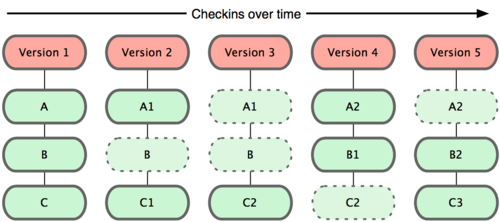
\includegraphics[width=0.7\linewidth]{../images/funcionamiento_git}
	\caption{Funcionamiento de Git en el versionado de archivos}
	\label{fig:funcionamiento_git}
	\end{figure}

	Dado que los dos utilizamos Windows y para tratar de manera más sencilla los archivos que íbamos cambiando y subiendo a la aplicación, nos creamos dos repositorios en GitHub, uno para la memoria y otro para la aplicación.
	
	Sabemos que no es muy habitual que la documentación de un proyecto se realice a través de un sistema distribuido, sin embargo nos facilitó enormemente la tarea de llevar los cambios al día.
	
	Para poder trabajar de una manera más óptima sobre la documentación con Git, partimos el documento inicial de la memoria en capítulos, cada uno se convierte en un .tex diferente, lo cual nos permite trabajar de manera independiente sobre cada capítulo y a la hora de subir los cambios minimizar el número de errores que se nos pudiesen dar al trabajar los miembros del equipo sobre esos mismos archivos.\\*
	
	Las divisiones que se hicieron en el documento, los sitúan en carpetas diferentes, con lo cual tenemos un .tex principal que es el que soporta toda la estructura de carpetas y archivos y es el que los configura (posee la mayor parte de los paquetes utilizados para tratar la estructura y aspecto del documento) y une, de manera que al compilar el archivo principal, se acaban compilando el resto de los archivos .tex que cuelgan de el.\\*
	
	Utilizamos PowerShell para Windows, que es una implementación de un interprete de comandos para Windows enfocado hacia Git, es decir que nos proporciona un entorno para que podamos escribir nuestras ordenes por linea de comandos y tratar de esa manera con nuestro repositorio Git
	
	\begin{figure}[H]
		\centering
		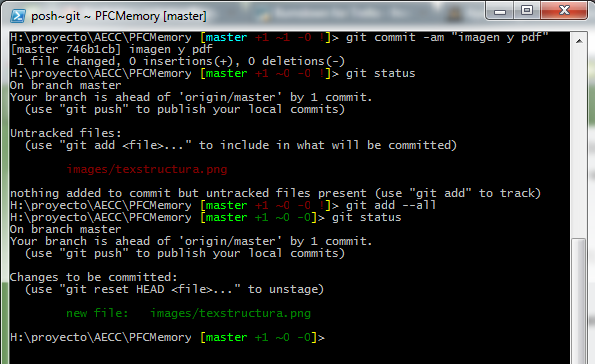
\includegraphics[width=0.9\linewidth]{../images/powershellcommit}
		\caption{PowerShell para Windows}
		\label{fig:powershellcommit}
	\end{figure}
	
	Windows PowerShell y en general Git, requieren un tiempo de aprendizaje, ya que la linea de comandos y los comandos en general no suelen ser demasiado amistosos con el usuario, y trabajar con ellos acarrea dificultades.
	
	No siempre todo lo que subimos encaja a la perfección y se pueden dar conflictos entre los archivos, de manera que hay que solucionarlos para dejar el repositorio estable.
	Estos conflictos se  pueden resolver de varias maneras posibles, puede ser a través de un merge, aceptando o eliminando los cambios locales, o modificando el resultado de lo que se va a subir, unificando el archivo que se va a quedar en el repositorio, se puede crear una nueva rama del proyecto (branch), o incluso se pueden apartar los cambios para seguir trabajando sobre la rama principal y hacer el commit de los mismos más tarde o desecharlos.
	
	\clearpage
	
	\begin{figure}[H]
		\centering
		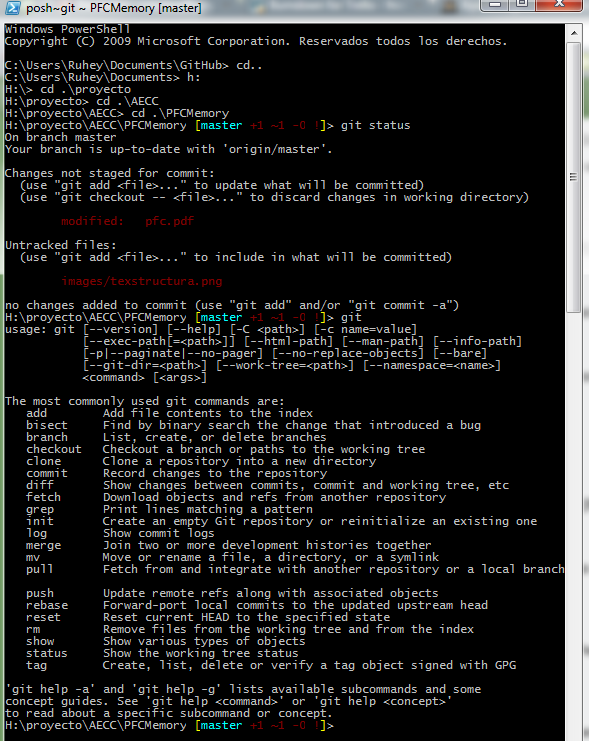
\includegraphics[width=0.8\linewidth]{../images/powerShell}
		\caption{PowerShell con los comandos más habituales a la hora de operar.}
		\label{fig:powershell}
	\end{figure}
	
	Como complemento a PowerShell, utilizamos como apoyo gráfico GitHub desktop, una aplicación gratuita que nos proporciona GitHub, y nos permite observar desde el propio Windows el estado del repositorio, los cambios que se han realizado, quien los ha realizado, etc.\\*
	
	Por contra, aunque sea muy visual y nos permita de un vistazo ver cuales son los archivos que se han modificado en el último commit, no tiene demasiadas opciones a la hora de interactuar con el repositorio, permite hacer un commit, desechar los cambios, hacer un revert (volver hacia atrás) y poco más.
	
	Es útil porque permite tener varios repositorios asociados y pasar de uno a otro es cosa de un click.
	

	\begin{figure}[H]
		\centering
		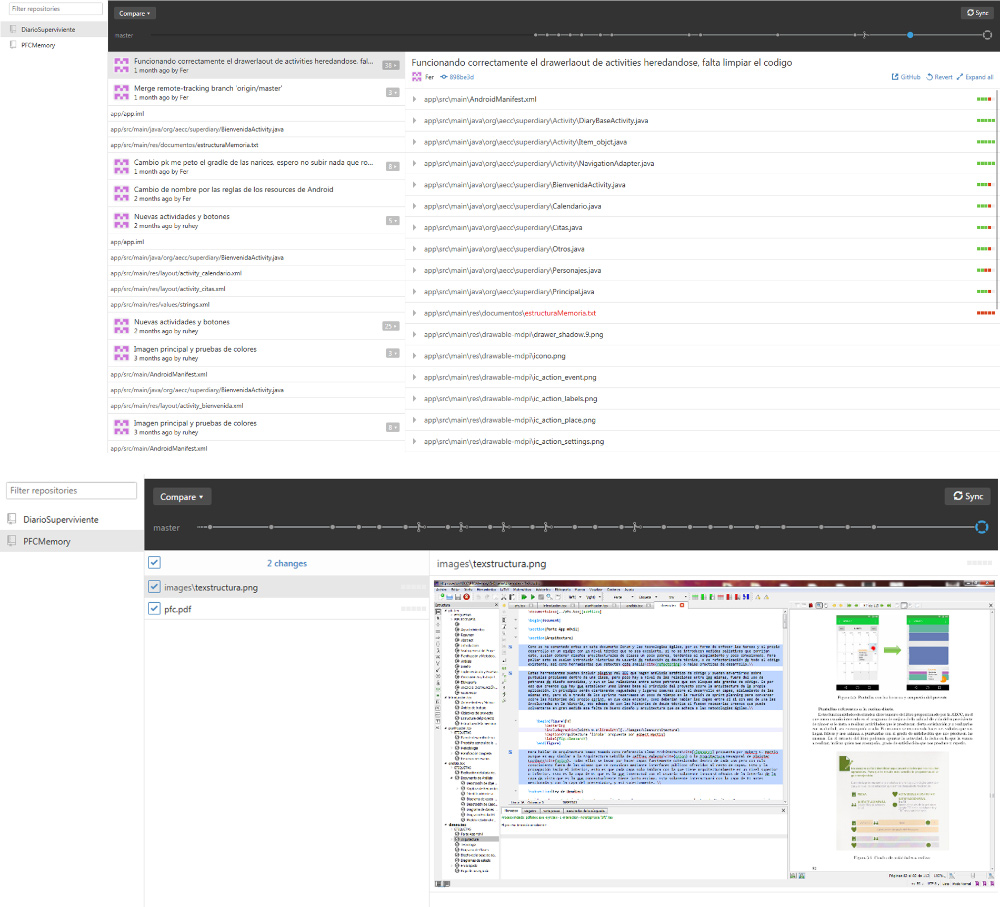
\includegraphics[width=1\linewidth]{../images/repositoriosGitHub}
		\caption{GitHub desktop, repositorios de la aplicación y de la memoria}
		\label{fig:ghdesktopA}
	\end{figure}

	Por ultimo vamos a hablar de las ventajas que nos reporta tener nuestra aplicación y memoria en GitHub, 
	\begin{itemize}
		\item Podemos decidir si el código va a ser publico o privado.
		\item Tiene un visor de código bastante avanzado, donde consultar en un instante el contenido de un determinado fichero, con su resaltado de sintaxis correspondiente para el lenguaje en el que esté escrito.
		Además de poder ver las diferentes versiones del mismo que se han subido, e incluso copiar porciones de código, etc.
		\item Dispone de bastantes herramientas que nos hacen muy fácil el trabajo en equipo, posibilidad de descargar el proyecto como un zip, una wiki, poder meter comentarios dentro del código, Una herramienta de revisión de código, donde se pueden añadir anotaciones en cualquier punto de un fichero, visor de ramas,...
		\item Herramienta de revisión de código, es decir puedes pedir modificar el código de los demás... o pueden mejorar tu propio código.
		\item Y por último y no menos importante, es gratis (siempre que sea código open source).
	\end{itemize}

	\begin{figure}[H]
		\centering
		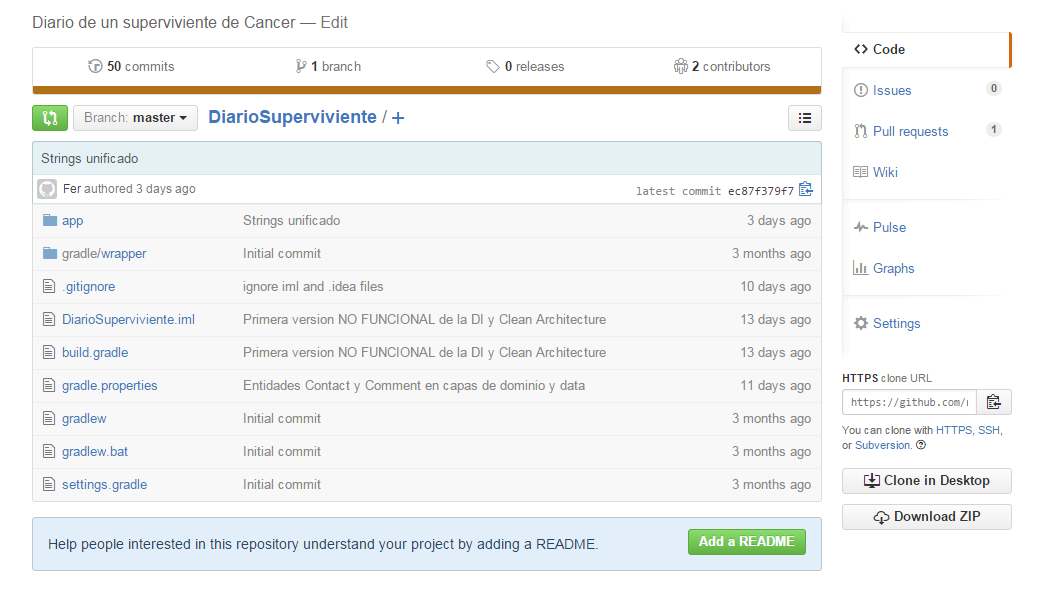
\includegraphics[width=1\linewidth]{../images/githubDiarioSuperviviente}
		\caption{Repositorio de GitHub desde la propia página web }
		\label{fig:ghweb}
	\end{figure}

	\clearpage
	
	\section{Pruebas}
	
	Hoy en día no se concibe un desarrollo de software sin disponer de pruebas o tester para poder asegurar la calidad del software y que este realiza las tareas para las que fue concebido correctamente y sin efectos laterales. Todo esto debido a que la complejidad del software desarrollado hoy día es de un orden de magnitud muy grande comparada con la de hace simplemente unos años.
	

	Es por ello que hoy en día la técnica de desarrollo que más adeptos consigue es el TDD (por su siglas en inglés de Test Driven Development) o Desarrollo Dirigido por Pruebas, en el cual ante una funcionalidad el desarrollador lo primero que ha de hacer es pensar en un test unitario y automático que falle. Después modificar el código todo lo rápido que pueda para hacer que dicho test automático pase a ser aprobado por la aplicación y por último refactorizar el software para mejorar el código antes escrito, eliminar duplicación, etc para volver al punto anterior en un proceso iterativo que acumulará test unitarios en estado de aprobación.\\* 
	
	\subsection{Tipos de pruebas}
		
		\begin{figure}[H]
			\centering
			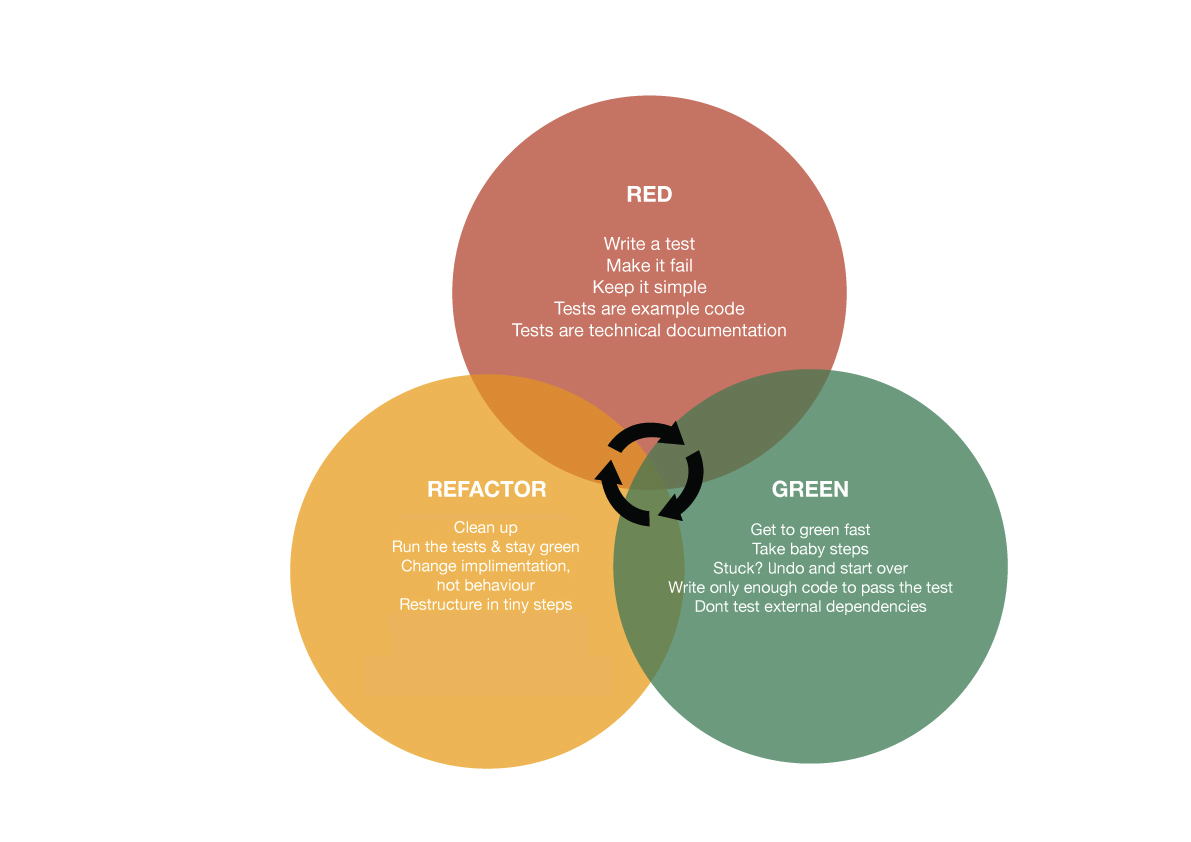
\includegraphics[width=1\linewidth]{../images/tdd_1}
			\caption{Ciclo de TDD con breves tips de cada una}
			\label{fig:Ciclo de TDD}
		\end{figure}
	
	De esta manera podemos obtener una confianza en que nuestro código sigue manteniendo la corrección, mientras vamos añadiendo funcionalidades a nuestra aplicación.\\*
	
	A tener en cuenta sobre esta técnica son los siguientes puntos:
		\begin{itemize}
			\item El test debe ser lo bastante pequeño para ser un test unitario pero a la vez añadir una funcionalidad que testar suficiente como para tener entidad propia. 
			\item Deben ejecutarse de manera rápida para poder ejecutar todos los test unitarios cada vez que se añade uno a la suite de casos de prueba.
			\item No genera evidencia de corrección en la aplicación por sí mismo.
			\item Probar de forma independiente la funcionalidad para la que fue diseñado. Casos de test interdependientes o que dependan del orden de ejecución de los mismos a menudo evidencian errores de diseño en la aplicación.
		\end{itemize}
	
	El proceso de desarrollo seguido llevando a cabo TDD da como resultado un software testable, desacoplado, y generalmente con las dependencias muy acotadas, aunque por contra como se ha mencionado en otras partes de este documento, arquitecturalmente suele desembocar en diseños poco cohesionados, ya que los test unitarios no suelen implicar refactorizar y mejorar el código de grandes bloques de clases, sino más bien de colaboradores directos. 
		 
	
	\subsection{ATDD y TDD}
	
	Como hemos hablado TDD es básicamente un proceso de desarrollo de software, de el se deriva una técnica, esta sí de pruebas propiamente dicha denominada ATDD, o Desarrollo Dirigido por Test de Aceptación. Esta técnica nace de la necesidad de obtener una evidencia de pruebas ante el software construido. Es el paso más corto desde el proceso de TDD. Se basa en que el cliente o product owner y el equipo definen en base a una historia de usuario, un test que dará como aceptado el software que ejecute dicho test de forma satisfactoria. Siguiendo la filosofía de TDD se basa en escribir un test junto al cliente a partir de la historia de usuario. Suele usarse el perfil del equipo más experto en pruebas para ayudar a diseñar el test junto al product owner. Después junto al equipo se piensa en como expandir el test, para finalmente pensar por parte de cada uno de los desarrolladores en como abordar partes de este Test de Aceptación, en test unitarios que abordar mediante el proceso de TDD. Cabe mencionar que este test se expresa mayormente en el lenguaje del equipo de desarrollo, por eso es necesario que el test de aceptación inicial se escriba en conjunto entre el product owner y alguien del equipo que domine su lenguaje. Aunque en un principio TDD necesita que los test sean automatizados, el proceso de ATDD no tiene por qué, aunque que este automatizado aumenta la eficiencia y utilidad de estos test así como de los test de regresión efectuados cada ronda de testing. 
		
	\subsection{BDD}
	
	BDD es otro proceso de testeo que se denomina así por sus siglas en inglés Behaviour Driven Developent, o desarrollo dirigido por comportamiento, es un proceso similar al de ATDD pero con la fundamental diferencia de que el lenguaje empleado en los test es el del dominio de la aplicación, y por lo tanto mucho mas cercano al product owner. Es por eso mucho más natural para él el tener que pensar en escribir un test que valide el comportamiento de una historia de usuario, aunque después este test sea más complicado de trasladar al TDD. El ciclo de BDD seria el mismo que el del TDD solamente que en cada iteración sobre un test de comportamiento implicaría varios ciclos de iteración sobre test de funcionalidad unitaria. Es deseable que estos test también estén automatizados y se lancen en el menor tiempo posible antes de cada compilación del código de la aplicación. Con estos ciclos de iteración a más alto nivel se consigue testar el comportamiento de la aplicación en algo evaluable y valioso para el product owner y forzar el refactorizado de código a más alto nivel para mejorar el diseño arquitectural de grandes bloques en principio menos interrelacionados que los que llevan a cabo los N test unitarios que subyacen al test de comportamiento.\\*
	
		\begin{figure}[H]
			\centering
			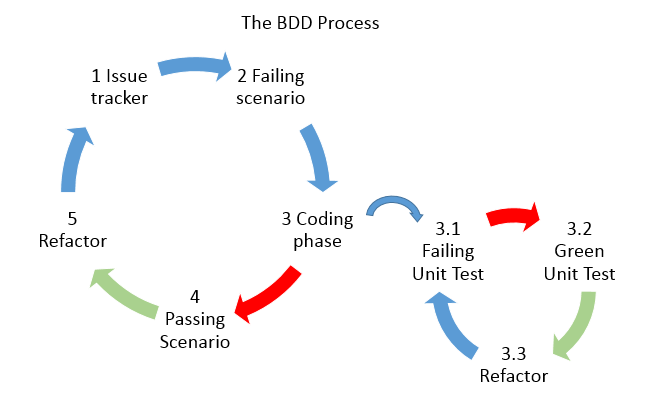
\includegraphics[width=1\linewidth]{../images/bdd1}
			\caption{Ciclos integrados de TDD y BDD }
			\label{fig:Ciclo de BDD y TDD}
		\end{figure}
	
	Esta cercanía al lenguaje de dominio de la aplicación hace que hoy día estos sean unos test muy apreciados por el product owner y que al equipo de desarrollo le obligan a testar no solo unitariamente el software de la aplicación, sino el comportamiento de los casos de uso descritos en la misma.\\* 
	
	\begin{figure}[H]
		\centering
		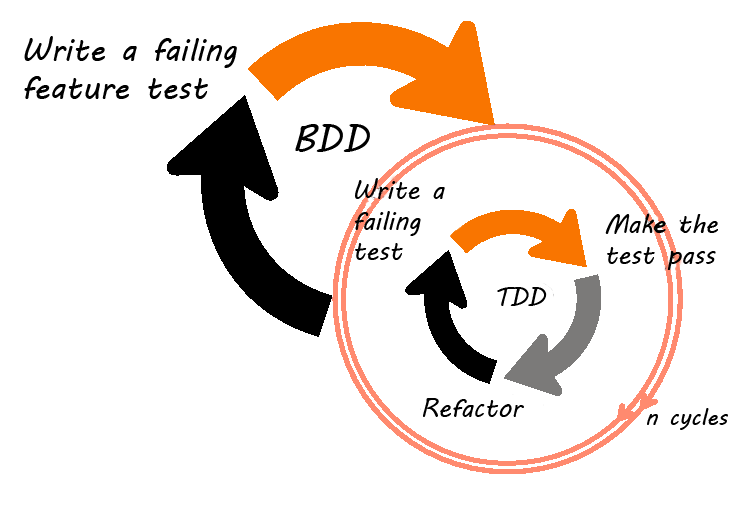
\includegraphics[width=1\linewidth]{../images/bdd2}
		\caption{Otra imagen de los ciclos integrados de TDD y BDD }
		\label{fig:Ciclo de BDD y TDD otro ejemplo}
	\end{figure}
		
	\subsection{Pruebas en el dispositivo}
	
	Por ultimo existe un bloque o tipo de test que son los que se realizan en el dispositivo. Estos se encargan sobre todo de testar la UI de la aplicación y que esta responde al comportamiento prefijado en los casos de uso y expresado en los test de comportamiento. Debido a las dependencias circulares a día de hoy no puede testarse en el mismo test el código del comportamiento de la app y el del SDK de Android. Por eso estos test de UI en dispositivo físico se separan del resto de test de la aplicación.\\*
	
	Debido a la gran variedad de dispositivos Android, por su abstracción sobre el hardware, es importante contar con la mayor base de terminales de diferentes características posibles. Además de esto es preciso poder contar con un sistema donde poder categorizar los usuarios de pruebas, así como recoger los ocasionales reportes que puedan enviarnos como feedback.\\*
	
	Como veremos en el siguiente punto esto puede lograrse entre otras maneras a través de la funcionalidad de versiones alpha y beta que la propia consola de desarrollador de la tienda Google Play Store nos ofrece. Con estas funcionalidades logramos disponer de una base de usuarios de test que muy probablemente ya estén familiarizados con la plataforma y no necesiten recibir más formación sobre ella.\\*
	
	\section{Puesta en producción}	
	
	El fin último de esta aplicación es que el público general se la descargue y use para mejorar su experiencia frente al cáncer. Por ello la misma debe estar en Play Store de Google, que es la tienda de aplicaciones más famosa y conocida del sistema operativo Android. Esta tienda pertenece a Google y para poder publicar en ella se debe hacer un pago único de 25 dólares. Tras esto se deben configurar las típicas pantallas de datos relativos al desarrollador email, web, dirección física, etc. Es recomendable rellenar estos datos pues los ofrece confianza a los usuarios, además de proveer a los mismos de toda una gama de formas de contactar con nosotros. Eso sí, si se proporciona un método de contacto ese método debe ser atendido. No hacerlo sería una publicidad y una imagen de marca horrorosa.\\*
	
	En la propia consola podemos crear la página para la o las aplicaciones, que será la que se vea en la web o al acceder a la tienda mediante la app. En ella se introducen datos sobre la propia app, así como vídeos, imágenes y demás media e información sobre la misma, de manera que el usuario pueda hacerse una idea bastante clara de lo que va a obtener al instalar la misma. Ademas estas páginas permiten realizar algo de posicionamiento de cara a ser encontrada más fácilmente, aunque para esto es más importante una buena valoración por cuantos más usuarios mejor. \\*
	
	Este sistema también permite la interacción con los usuarios. Mediante el sistema de valoración de apps podemos responder a los usuarios, si es que estos plantean errores o bugs.\\* 
	
	\begin{figure}[H]
		\centering
		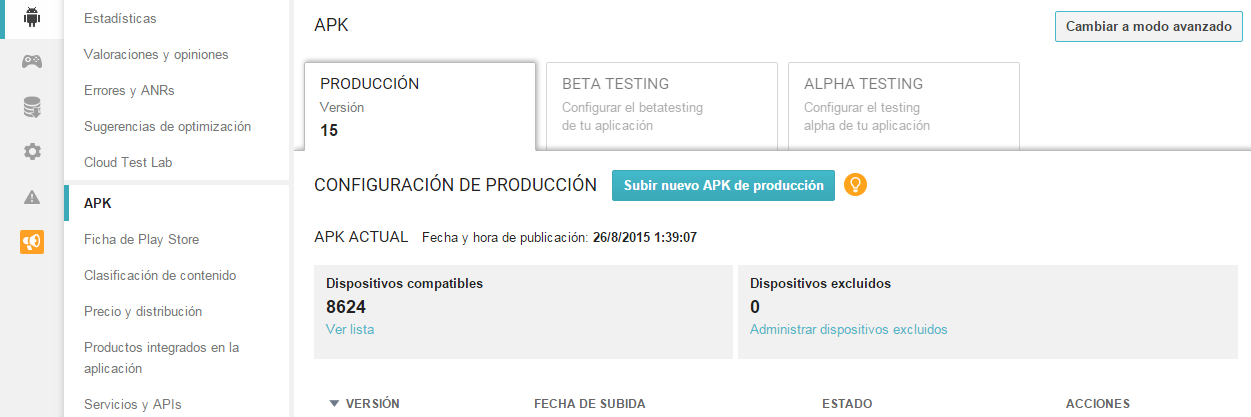
\includegraphics[width=1\linewidth]{../images/consola_apk}
		\caption{Consola de Play Store, mostrando gestión de APK y versiones beta y alpha }
		\label{fig:Consola de Play Store: APK}
	\end{figure}
	
	En la sección de APK, el binario a distribuir, podemos tener varios binarios en espera de poner en producción, así como activar la característica de utilizar versiones alpha y beta. 
	
\end{document}